\chapter{Training Spiking Deep Learning Models On-line Using Spike-based Rate Multiplication (SRM)}
\label{cha:sdlm}
%Paragraph One: LINK
%Make a connection to what has immediately gone before. Recap the last chapter. In the last chapter I showed that… Having argued in the previous chapter that… As a result of x, which I established in the last chapter….. It is also possible to make a link between this chapter and the whole argument… The first step in answering my research question (repeat question) .. was to.. . In the last chapter I …
Having argued in the previous chapter that it is feasible to construct deep SNNs off-line by training DNN with specific activation function.
This Chapter continues the hot topic of deep SNNs and takes extra step forward to biologically inspired, on-line, spike-based training.

%Paragraph Two: FOCUS
%Now focus the reader’s attention on what this chapter is specifically going to do and why it is important. In this chapter I will examine.. I will present… I will report … This is crucial in (aim of thesis/research question) in order to….
In this Chapter We will present the method, Spike-based Rate Multiplication (SRM).
This algorithm successfully transfers multiplication operations to possibility of some specific firing events of a pair of rate-coded spike trains.
Moreover, these firing events can be captured with Synaptic-Time-Dependent Plasticity (STDP) rule thus to update the weights accordingly in an on-line, event-based, and biologically-plausible manner.
Such weight update well fits the conventional unsupervised deep learning modules: such as Autoencoders (AE) and Restricted Boltzmann Machines (RBMs), where multiplication of the neural outputs is the main operation.
It is crucial to provide deep SNNs with effective on-line training algorithm not only for building successful spike-based object recognition applications, but also for better power efficiency and scalability when training on neuromorphic hardware.


%Paragraph Three: OVERVIEW
%The third paragraph simply outlines the way that you are going to achieve the aim spelled out in the previous paragraph. It’s really just a statement of the contents in the order that the reader will encounter them. It is important to state these not simply as topics, but actually how they build up the internal chapter argument… I will begin by examining the definitions of, then move to seeing how these were applied… I first of all explain my orientation to the research process, positioning myself as a critical scholar.. I then explain the methodology that I used in the research, arguing that ethnography was the most suitable approach to provide answers to the question of… 
%https://patthomson.net/2014/01/16/connecting-chapterschapter-introductions/
We first of all explore the research question of on-line, event-based deep SNN training in the literature.
We then describe SRM in mathematical expression, and explain the factors influencing the accuracy of the method and the factors not. 
Afterwards we argue why the learning algorithm is proper to train spiking Autoencoders (SAEs) and Spiking Restricted Boltzmann Machines (SRBM).
During the research we encountered the problem introduced by the correlated spikes, therefore we also propose solutions to decorrelate spike trains in Section~\ref{sec:problem}. 
Finally the detailed comparison of the traditional training and SRM learning on MNIST dataset demonstrates the equivalent learning ability and shows similar even surpassing recognition and reconstruction capability of SRM.


\section{Related Works}
%To start with evidence of energy efficiency: maybe should refer to Chapter 2 or 1.
The current trend towards training deep SNNs on line using biologically-plausible learning methods is promising due to its potential benefit on low-energy hardware implementation.
%0. Dan Neil: Online Learning in Event-based Restricted Boltzmann Machines
The first on-line training algorithm of unsupervised learning is event-based contrastive divergence (evtCD)~\cite{neil2013online} for SRBM, which firstly found out the feasibility of applying STDP rule to approximate CD algorithm.
To review the algorithm of training RBMs, please refer to Section~\ref{sec:rbm}.
The method divided the learning process into potentiating and depression parts, which formed the basic design of related research.
As an initial attempt the mathematical analysis was mainly ignored, thus the best classification performance achieved was only about 81.5\% using purely spiking neurons.
%1. Neftci
\cite{neftci2013event} derived the division of potentiating and depression parts of CD algorithm, but conduct them both on the same neural populations which was more biologically plausible.
Therefore, a global signal was needed to differentiate the potentiating and depression process.
And the rhythmic oscillation of these processes generated the particular form of neural sampling~\cite{petrovici2013stochastic}.
The work focused on the statistical aspect of the event-driven sampling, and was extended to the later work on Synaptic Sampling Machines (S2Ms)~\cite{neftci2016stochastic} with stochastic synapses.
The classification accuracy of MNIST was 91.9\%, 1.7\% lower than the conventional RBM.
Similar work of Dan's SRBM training, \cite{burbank2015mirrored} applied STDP rule to train SAEs in very much biologically-plausible manner.
This work aimed at constructing artificial machine learning algorithm closely to biology, whereas the other works above focused on training spiking deep learning modules with equivalent recognition capability as alternative deep learning methods.

%4. remote (ReSuMe)
The work we propose was mostly inspired from the supervised time-based spiking learning rule~\cite{ponulak2010supervised}, ReSuMe, where the output spikes of a post-synaptic neuron were trained to generate at expected time points with certain input pattern injected to the pre-synaptic neurons, see Figure~\ref{fig:resume}.
The teaching signal always potentiates the synaptic strength according to the exponential STDP curve on the time difference between the teaching spike and the pre-synaptic spike; and the output spikes of the post-synaptic neuron always depress the connection.
Thus, if an output spike fires earlier than the teaching spike the weight will depress more than it potentiate, thus the output spike should be delayed the next trial; and the vice versa if the post-synaptic neuron spikes later.
Therefore, the weight stays constant only when the output spikes fire coincidently with the teaching signal.
\begin{figure}
	\centering
	\includegraphics[width=0.4\textwidth]{pics_sdlm/ReSuMe.pdf}
	\caption{Network architecture of a pair of pre- and post-synaptic neurons trained by ReSuMe~\cite{ponulak2010supervised} with a teaching signal.}
	\label{fig:resume}
\end{figure}

The basic idea of the proposed method is to provide equivalent learning rule as ReSuMe on rate-encoded SNNs.
The objective is to supervise the post-synaptic neuron to fire at the frequency of the teaching spike train. 
Accordingly, the weight decreases if the output neuron fires stronger than the teaching neuron, and vice versa.
The synaptic strength stops changing as the output neuron fires at the same frequency of the teaching signal.
The algorithm is simply divided into spike-based rate multiplication (SRM) problems, and we will demonstrate the SRM method in following Section~\ref{sec:SRM}.
The learning rule can be easily applied to SAEs if we use input spikes as teaching signals to the visible units, moreover the CD algorithm of training SRBMs is still not more than two operations of SRMs.
Section~\ref{sec:dSNN} explains the specific training on SAEs and SRBMs in detail.
 

\section{Spike-based Rate Multiplication (SRM)}
\label{sec:SRM}
If we see \textit{pre}, \textit{post} and \textit{teach} as vectors individually, and \textit{w} as a weight matrix of the all-to-all connections between \textit{pre} and \textit{post} in Figure~\ref{fig:resume}, the network will form the Adaline (Adaptive Linear Element) which is a single-layered ANN.
The learning algorithm was named after the researcher Widrow-Hoff:
\begin{equation}
\Delta w = \eta (teach - post)pre,
\end{equation}
which is equivalent to Stochastic Gradient Descent~(SGD) in Multi-Layered Perceptrons~(MLPs).
The right hand of the equation can be seen as two operations of multiplication, $teach \times pre$ and $post \times pre$, times the constant learning rate, $\eta$.

SRM provides the solution to present numeric multiplication $c=ab$ with rate-based spike trains.
First of all, the multiplier $a$ and the multiplicand $b$ are encoded into Poisson spike trains $s_a=\{s_a(1),s_a(2),...,s_a(T)\}$ and $s_b=\{s_b(1),s_b(2),...,s_b(T)\}$ in the 1~ms resolution, where $s(t)=1$ indicates a spike in the $t$th~ms and $s(t)=0$ means none.
Secondly, a Poisson generator fires a sequence of spike train according to its firing rate, $\lambda$~Hz, which is assigned linearly to the original multiplier/multiplicand by a factor of $K$.
Hence, the firing rate ($\lambda_x$) of the Poisson generator is $K$ times of the numerical value x, and can be approximated by the average spike count, $N_T(s_x)$, of the generated spike train $s_x$ over time length of $T$:
\begin{equation}
\lambda_x = Kx \approx N_T(s_x) = \frac{1000}{T} \sum_{t=1}^{T} s_x(t) ,
\end{equation} 
and 1000 is the scale factor for scaling frequency per millisecond to per second.
Significantly, the approximation is more accurate as the observing time ($T$) grows since more spikes are generated over time and the average spike count becomes more reliable.
Thirdly, assuming $s_a$ and $s_b$ are independent Poisson spike trains the core definition of the rate multiplication of the pair of spike trains is as follows:
\begin{equation}
\lambda_a \lambda_b \approx N_{T_1}(s_a)N_{T_2}(s_b)= 10^6 \frac{\sum_{t_a=1}^{T_1}s_a(t_a)}{T_1}  \frac{\sum_{t_b=1}^{T_2} s_b(t_b)}{T_2}.
\label{equ:mul}
\end{equation} 

Finally, if we combine the concept of the STDP learning window to equation~\ref{equ:mul}, the length of the observing time on $s_b$ shrinks to a fix-length windowing period, $\tau_{win}$.
Consequently, the rate multiplication can be conducted within only the local events in term of time, although the accuracy may drop.
The rate multiplication is then approximated by:
\begin{equation}
\lambda_a \lambda_b \approx \frac{10^6}{\tau_{dur} \tau_{win}} \sum_{t=1}^{\tau_{dur}} [s_a(t) \sum_{t_b=t}^{t+\tau_{win}} s_b(t_b)],
\end{equation} 
where $\tau_{dur}$ replaces $T$ to represent the length of generated spike trains during SNN simulation.
The weight rise/drop according to a rectangular STDP curve can detect the spike events of a pair of spike trains when post-synaptic spike occurs no later than $\tau_{win}$, see Figure~\ref{fig:rtg_stdp}.
Therefore, the overall weight change during time $\tau_{dur}$ indicates the rate multiplication, and is decried by SRM:
\begin{equation}
\begin{aligned}
\Delta w = SRM(s_a, s_b) &= \eta_s \sum_{t=1}^{\tau_{dur}} [s_a(t) \sum_{t_b=t}^{t+\tau_{win}} s_b(t_b)] \text{, and}\\
c=ab=\frac{\lambda_a \lambda_b}{K^2} &\approx \frac{10^6}{K^2 \tau_{dur} \tau_{win}} \sum_{t=1}^{\tau_{dur}} [s_a(t) \sum_{t_b=t}^{t+\tau_{win}} s_b(t_b)] \\
&\approx  \frac{10^6 SRM(s_a, s_b)}{K^2 \tau_{dur} \tau_{win}  \eta_s}.
\end{aligned}
\label{equ:srm}
\end{equation} 
\begin{figure}
	\centering
	\includegraphics[width=0.4\textwidth]{pics_sdlm/stdp.pdf}
	\caption{Rectangular STDP curve.
		If the time difference of the post-synaptic spike and the pre-synaptic spike lies in the window on $\tau_{win}$, then the synaptic weight will increase by $\eta_s$.}
	\label{fig:rtg_stdp}
\end{figure}

We can adjust $\eta_s$ to $ K^2 \tau_{dur} \tau_{win}10^{-6}$ to make $ab = \Delta w$.
In terms of the Widrow-Hoff learning algorithm, $\eta_s$ is set to be:
\begin{equation}
	\eta_s=
    \left\{
    \begin{aligned} 
    \eta K^2 \tau_{dur} \tau_{win}10^{-6}, &\text{ when calculating } \eta teach \times pre\\
    - \eta K^2 \tau_{dur} \tau_{win}10^{-6}, &\text{ when calculating } \eta post \times pre
    \end{aligned}
    \right.
    \label{equ:eta_s}
\end{equation}
In Section~\ref{sec:AE}, we demonstrate how Widrow-Hoff algorithm successfully applies to training AEs (see Equation~\ref{equ:ae_widrow_hoff}) and in Section~\ref{subsec:SAE} we describe the implementation of SRM algorithm to deep learning models of spiking AEs and RBMs.

Last but not least, we state the property of SRM algorithm:
\begin{itemize}
	\item the accuracy of SRM is mainly controlled by $\tau_{dur}$ and $\tau_{win}$, where longer spike trains and longer STDP window expresses the rate more reliable.
	\item in spiking neural network both the multiplier and the multiplicand can only be presented as rates, which is positive.
	Thus negative product is applied with weight decrease, $-\eta_s$. 
	\item the multiplier and the multiplicand are interchangeable due to the independence of the spike trains. 
	\item the accuracy is independent of neural model and synaptic model because the calculation relies on the firing rate only.
\end{itemize}
\section{Training Deep SNNs}
\label{sec:dSNN}
The Section conducts experiments to compare conventional deep learning modules to spiking versions of them.
To start with, AEs and RBMs are trained with clean numerical values, and then with noisy values which are generated by presenting the original values with Poisson spike trains and transferring the spike counts back to numerical values.
These experiments run as baselines to compare with spike based training on the features of weights' convergence, reconstruction error and neurons' activities.

There are two set-ups of the same network architecture where ten visible neurons connect to the layer of ten hidden neurons symmetrically with all-to-all weights: (1)~the values of all the input data are 1, $input_1 = [1, 1, 1,...,1]$; and (2)~the input data range from 0.1 to 1 linearly with step of 0.1, $input_2 = [0.1, 0.2, 0.3,...,1]$.
These two experiments provide a close observation on the weight updates given the constant input values.
And Experiment I shows how the network responds to a same input value 1, and reconstructs it; while Experiments II can demonstrate the influence of ranging input values, more importantly how firing rate may affect the corresponding SNN.

Following the experiments of conventional models, we propose the training methods of SAEs and SRBMs in detail.
The same experiments are then applied to the on-line and spike-based algorithm.

\subsection{Autoencoders (AEs)}
\label{sec:ae}
Using ReLU and Equation~\ref{equ:ae_widrow_hoff}, we can easily train a layer of AEs with a small network size of 10 visible units and 10 output units.
The initial weights are randomly generated with unified distribution from 0 to 0.01, and the learning rate, $\eta$, is set to 0.001.
We keep the same initial weights for all the experiments thus to provide an accurate comparison on the weight update.
The input vector, seen as an image, repeatedly feed into the network for $5,000$ times and Figure~\ref{fig:ae_orig} shows the dynamics of the AE as more repeating images present through training.

\begin{figure}
	\centering
	\begin{subfigure}[t]{0.45\textwidth}
		\includegraphics[width=\textwidth]{pics_sdlm/20_exp_AE/exp1_weights_non.pdf}
		\caption{Weights of Exp1}
	\end{subfigure}
	\begin{subfigure}[t]{0.45\textwidth}
		\includegraphics[width=\textwidth]{pics_sdlm/20_exp_AE/exp2_weights_non.pdf}
		\caption{Weights of Exp2}
	\end{subfigure}
	\begin{subfigure}[t]{0.45\textwidth}
		\includegraphics[width=\textwidth]{pics_sdlm/20_exp_AE/exp1_recon_non.pdf}
		\caption{Reconstruction of visible units in Exp1}
	\end{subfigure}
	\begin{subfigure}[t]{0.45\textwidth}
		\includegraphics[width=\textwidth]{pics_sdlm/20_exp_AE/exp2_recon_non.pdf}
		\caption{Reconstruction of visible units in Exp2}
	\end{subfigure}\\
	\begin{subfigure}[t]{0.45\textwidth}
		\includegraphics[width=\textwidth]{pics_sdlm/20_exp_AE/exp1_hid_non.pdf}
		\caption{Output of hidden units in Exp1}
	\end{subfigure}
	\begin{subfigure}[t]{0.45\textwidth}
		\includegraphics[width=\textwidth]{pics_sdlm/20_exp_AE/exp2_hid_non.pdf}
		\caption{Output of hidden units in Exp2}
	\end{subfigure}\\
	\begin{subfigure}[t]{0.45\textwidth}
		\includegraphics[width=\textwidth]{pics_sdlm/20_exp_AE/exp1_loss.pdf}
		\caption{Output of hidden units in Exp1}
	\end{subfigure}
	\begin{subfigure}[t]{0.45\textwidth}
		\includegraphics[width=\textwidth]{pics_sdlm/20_exp_AE/exp2_loss.pdf}
		\caption{Output of hidden units in Exp2}
	\end{subfigure}
	\caption{Changes of weights, output of visible and hidden units, and mean squared error (loss) during the AE training of the reconstruction tests. 
		Experiments 1) 10 visible units fully connected to 10 hidden units with input data of all 1s; 2) same network fed with 10 values distribute linearly from 0.1 to 1.}
	\label{fig:ae_orig}
\end{figure}

In order to compare all the experiments following, we demonstrate the results in the same figure template:
(a) and (b) depict the weight change of the two experiment set-ups (Exp1 and Exp2) which is the most important output of a training method;
(c) and (d) visually display the output of the visible units, the reconstruction of the input vector;
(e) and (f) draw the output of the hidden units during training and assist the observation on weight change and the reconstruction;
(g) and (h) intuitively show the loss (mean squared error) and validate how well the reconstructions are.


For Exp1, the reconstruction loss reduces exponentially to the limit of the computer's float precision (Figure~\ref{fig:ae_orig}(g)), and reaches $10^{-4}$ using about 600 steps, and from that point the weights, visible reconstruction, and the output of the hidden units nearly stabilise, see Figure~\ref{fig:ae_orig}(a,c,e).
With differentiate input values in Exp2, the training runs slower taking about $1,400$ steps to reach the same performance of $10^{-4}$ loss (Figure~\ref{fig:ae_orig}(h)).
The reason of the slower training comes to the weaker input and it also makes the output of the hidden units lower than Exp1, see Figure~\ref{fig:ae_orig}(f), thus the positive part of the weight change, $\eta h_i v_j$, is much weakened. 
The reconstructions, shown in Figure~\ref{fig:ae_orig}(d), of smaller values stabilise earlier than the ones of higher values, since the higher output of the reconstruction requires stronger weights and more accumulated weight updates. 
\begin{figure}
	\centering
	\begin{subfigure}[t]{0.45\textwidth}
		\includegraphics[width=\textwidth]{pics_sdlm/21_exp_AE_noise/exp1_weights_s.pdf}
		\caption{Weights of Exp1}
	\end{subfigure}
	\begin{subfigure}[t]{0.45\textwidth}
		\includegraphics[width=\textwidth]{pics_sdlm/21_exp_AE_noise/exp2_weights_s.pdf}
		\caption{Weights of Exp2}
	\end{subfigure}
	\begin{subfigure}[t]{0.45\textwidth}
		\includegraphics[width=\textwidth]{pics_sdlm/21_exp_AE_noise/exp1_recon_s.pdf}
		\caption{Reconstruction of visible units in Exp1}
	\end{subfigure}
	\begin{subfigure}[t]{0.45\textwidth}
		\includegraphics[width=\textwidth]{pics_sdlm/21_exp_AE_noise/exp2_recon_s.pdf}
		\caption{Reconstruction of visible units in Exp2}
	\end{subfigure}\\
	\begin{subfigure}[t]{0.45\textwidth}
		\includegraphics[width=\textwidth]{pics_sdlm/21_exp_AE_noise/exp1_hid_s.pdf}
		\caption{Output of hidden units in Exp1}
	\end{subfigure}
	\begin{subfigure}[t]{0.45\textwidth}
		\includegraphics[width=\textwidth]{pics_sdlm/21_exp_AE_noise/exp2_hid_s.pdf}
		\caption{Output of hidden units in Exp2}
	\end{subfigure}\\
	\begin{subfigure}[t]{0.45\textwidth}
		\includegraphics[width=\textwidth]{pics_sdlm/21_exp_AE_noise/exp1_loss_s.pdf}
		\caption{Output of hidden units in Exp1}
	\end{subfigure}
	\begin{subfigure}[t]{0.45\textwidth}
		\includegraphics[width=\textwidth]{pics_sdlm/21_exp_AE_noise/exp2_loss_s.pdf}
		\caption{Output of hidden units in Exp2}
	\end{subfigure}
	\caption{Changes of weights, output of visible and hidden units, and mean squared error (loss) during the AE training of the noisy reconstruction tests. 
		Experiments 1) 10 visible units fully connected to 10 hidden units with the count of Poisson spikes firing at 100~Hz which lasted 100~ms; 2) same network fed with spike count of Poisson spikes at firing rate ranging from 10~Hz to 100~Hz.}
	\label{fig:ae_noise}
\end{figure}

The same experiments are repeated with noisy training and testing data to provide a fair comparison with the spike-based deep learning modules, see Figure~\ref{fig:ae_noise}.
The noisy data is gathered from the SNN experiments in Section~\ref{subsec:SAE}, and the corresponding SRM parameters are listed in Table~\ref{tbl:srm}.
All the SNN experiments use the same training and testing Poisson spike trains for the purpose of unified experimental environment.
The firing rates of the input values are scaled up by the factor $K = 100$, thus $\lambda_1 = [100, 100, 100, ..., 100]$ Hz and $\lambda_2 = [10, 20, 30, ..., 100]$ Hz.
The spike count $c$ of a generated Poisson spike train then transformed to the noisy input, $c/(\tau_{dur} * K)$.
The length of spike trains $\tau_{dur}$ is 0.1~s when training, and 1~s for testing.
The longer the spike trains are, less noisy the spike counts become.
The noisy input can be seen as distorted data by adding Gaussian noise on the original value.
Hence, the noisy training input adds the clean data a Gaussian noise with -0.05 mean and 0.29 variance for Exp1, and -0.02 mean and 0.22 variance for Exp2;
while in terms of testing data, see Figure~\ref{fig:noise_input}, the means of the noise are the same, but the variances are much smaller: 0.09 for Exp1 and 0.07 for Exp2.
\begin{figure}
	\centering
	\begin{subfigure}[t]{0.45\textwidth}
		\includegraphics[width=\textwidth]{pics_sdlm/21_exp_AE_noise/exp1.pdf}
		\caption{Input images of Exp1}
	\end{subfigure}
	\begin{subfigure}[t]{0.45\textwidth}
		\includegraphics[width=\textwidth]{pics_sdlm/21_exp_AE_noise/exp2.pdf}
		\caption{Input images of Exp2}
	\end{subfigure}
	\caption{Noisy input gathered from Poisson spike trains.}
	\label{fig:noise_input}
\end{figure}


Figure~\ref{fig:ae_noise} shows the effect of the noisy input, although the training stabilises at roughly the same time point.
First of all, it generates slight waves on the weight changes.
Secondly, the reconstruction and the output of the hidden units are noisy comparing to the training and testing on clean data, however the noise are much reduced from the noisy input data (Figure~\ref{fig:noise_input}). 
Finally, the loss keeps in a certain level and stops dropping.
The loss of Exp2 is lower than Exp1, in other words the reconstruction on Exp2 are closer to the input data.
It is mainly caused the weaker noise level on the smaller input values that the data is less noisy in Exp2 in average. 
\begin{figure}
	\centering
	\begin{subfigure}[t]{0.45\textwidth}
		\includegraphics[width=\textwidth]{pics_sdlm/30_exp_RBM/exp1_weights_non.pdf}
		\caption{Weights of Exp1}
	\end{subfigure}
	\begin{subfigure}[t]{0.45\textwidth}
		\includegraphics[width=\textwidth]{pics_sdlm/30_exp_RBM/exp2_weights_non.pdf}
		\caption{Weights of Exp2}
	\end{subfigure}
	\begin{subfigure}[t]{0.45\textwidth}
		\includegraphics[width=\textwidth]{pics_sdlm/30_exp_RBM/exp1_recon_non.pdf}
		\caption{Reconstruction of visible units in Exp1}
	\end{subfigure}
	\begin{subfigure}[t]{0.45\textwidth}
		\includegraphics[width=\textwidth]{pics_sdlm/30_exp_RBM/exp2_recon_non.pdf}
		\caption{Reconstruction of visible units in Exp2}
	\end{subfigure}\\
	\begin{subfigure}[t]{0.45\textwidth}
		\includegraphics[width=\textwidth]{pics_sdlm/30_exp_RBM/exp1_hid_non.pdf}
		\caption{Output of hidden units in Exp1}
	\end{subfigure}
	\begin{subfigure}[t]{0.45\textwidth}
		\includegraphics[width=\textwidth]{pics_sdlm/30_exp_RBM/exp2_hid_non.pdf}
		\caption{Output of hidden units in Exp2}
	\end{subfigure}\\
	\begin{subfigure}[t]{0.45\textwidth}
		\includegraphics[width=\textwidth]{pics_sdlm/30_exp_RBM/exp1_loss.pdf}
		\caption{Output of hidden units in Exp1}
	\end{subfigure}
	\begin{subfigure}[t]{0.45\textwidth}
		\includegraphics[width=\textwidth]{pics_sdlm/30_exp_RBM/exp2_loss.pdf}
		\caption{Output of hidden units in Exp2}
	\end{subfigure}
	\caption{Changes of weights, output of visible and hidden units, and mean squared error (loss) during the nRBM training of the reconstruction tests. 
		Experiments 1) 10 visible units fully connected to 10 hidden units with input data of all 1s; 2) same network fed with 10 values distribute linearly from 0.1 to 1.}
	\label{fig:rbm_orig}
\end{figure}

\begin{figure}
	\centering
	\begin{subfigure}[t]{0.45\textwidth}
		\includegraphics[width=\textwidth]{pics_sdlm/31_exp_RBM_noise/exp1_weights_s.pdf}
		\caption{Weights of Exp1}
	\end{subfigure}
	\begin{subfigure}[t]{0.45\textwidth}
		\includegraphics[width=\textwidth]{pics_sdlm/31_exp_RBM_noise/exp2_weights_s.pdf}
		\caption{Weights of Exp2}
	\end{subfigure}
	\begin{subfigure}[t]{0.45\textwidth}
		\includegraphics[width=\textwidth]{pics_sdlm/31_exp_RBM_noise/exp1_recon_s.pdf}
		\caption{Reconstruction of visible units in Exp1}
	\end{subfigure}
	\begin{subfigure}[t]{0.45\textwidth}
		\includegraphics[width=\textwidth]{pics_sdlm/31_exp_RBM_noise/exp2_recon_s.pdf}
		\caption{Reconstruction of visible units in Exp2}
	\end{subfigure}\\
	\begin{subfigure}[t]{0.45\textwidth}
		\includegraphics[width=\textwidth]{pics_sdlm/31_exp_RBM_noise/exp1_hid_s.pdf}
		\caption{Output of hidden units in Exp1}
	\end{subfigure}
	\begin{subfigure}[t]{0.45\textwidth}
		\includegraphics[width=\textwidth]{pics_sdlm/31_exp_RBM_noise/exp2_hid_s.pdf}
		\caption{Output of hidden units in Exp2}
	\end{subfigure}\\
	\begin{subfigure}[t]{0.45\textwidth}
		\includegraphics[width=\textwidth]{pics_sdlm/31_exp_RBM_noise/exp1_loss_s.pdf}
		\caption{Output of hidden units in Exp1}
	\end{subfigure}
	\begin{subfigure}[t]{0.45\textwidth}
		\includegraphics[width=\textwidth]{pics_sdlm/31_exp_RBM_noise/exp2_loss_s.pdf}
		\caption{Output of hidden units in Exp2}
	\end{subfigure}
	\caption{Changes of weights, output of visible and hidden units, and mean squared error (loss) during the nRBM training of the noisy reconstruction tests. 
		Experiments 1) 10 visible units fully connected to 10 hidden units with the count of Poisson spikes firing at 100~Hz which lasted 100~ms; 2) same network fed with spike count of Poisson spikes at firing rate ranging from 10~Hz to 100~Hz.}
	\label{fig:rbm_noise}
\end{figure}

\subsection{Noisy Restricted Boltzmann Machines (nRBMs)}
Instead of using binary units in RBM, we employ noisy ReLU (NReLU) units to construct nRBM which is closer to biology and performs better in classification tasks~\cite{nair2010rectified}.
Leaving the learning algorithm unchanged, see Algorithm~\ref{alg:rbm} in Section~\ref{sec:rbm}, the new sampling method NReLU is equivalent to generating multiple samples in the meantime and averaging them: $max(0, x+\mathcal{N}(0, \sigma(x))$.
The lower the variance of the normal distribution is, it means more samples are taken for averaging.
To put it differently, zero variance (equivalent to ReLU) is used when unlimited samples are generated, but at the same time the sampling itself loses the randomness.
In our experiments the variance of the normal distribution used in NReLU is 0.1 during training.
While in testing, we use ReLU for the deterministic reconstructions. 
To keep the similar network architecture and the learning rule with AEs, we use RBM with zero bias as well.
Thus the weight updating rule in Algorithm~\ref{alg:rbm} can be simplified as:
\begin{equation}
\Delta w_{ij} = \eta (h_iv_j - h'_iv'_j),
\label{equ:rbm}
\end{equation} 
where $h'_i$ and $v'_j$ is a pair of Gibbs sampling.

Figure~\ref{fig:rbm_orig} demonstrates the training process and the testing result of nRBM, both experiments stabilise earlier than AE training: about 400 and $1,000$ steps respectively.
Due to randomness of the sampling in nRBM, there are noisy waves adding on the weights during training, the reconstructions and the output of hidden units in deterministic testing, and the loss stops declining around $10^{-4}$.

The same experiments are also carried out with the identical noisy input described above, see Figure~\ref{fig:rbm_noise}.
The weight change is slightly more noisy than the experiments on clean data.
But the noise are more obvious on the output of the visible reconstruction and the hidden units.
The same effect of the noisy input data can be found in Figure~\ref{fig:ae_noise} that the noise on the reconstruction is much reduced comparing to the input data and the loss remains about $10^{-2}$ and $10^{-2.5}$ after the stabilisation, although it takes less time for nRBM to converge than AE.


\subsection{Training Spiking Autoencoders (SAEs)}
\label{subsec:SAE}
Equation~\ref{equ:ae_widrow_hoff} states the learning rule of AE, which can be approximated by adding up a positive SRM and a negative SRM.
The weight increase takes place in the positive STDP learning between the neurons of the input ($\bf{v}$) and the hidden units ($\bf{h}$); and the weight decrease carries out in the negative STDP learning between the reconstruction ($\bf{v'}$) and the hidden neurons ($\bf{h}$).
Figure~\ref{fig:AE} shows the network architecture of an SAE where the hidden units connect to the reconstruction neurons with the weight matrix $\bf{w}$ and the input neurons feedforward to the hidden layer with the transposed tied weights $\bf{w}^\textrm{T}$.
The shared weights, three individual populations of neurons build the training network of an SAE.

\begin{figure}
	\centering
	\includegraphics[width=0.8\textwidth]{pics_sdlm/rSTDP.pdf}
	\caption{How SRM works in training spiking Autoencoders.}
	\label{fig:rSTDP}
\end{figure}

Figure~\ref{fig:rSTDP} illustrates the learning mechanism of the SAE architecture by giving an example of one hidden neuron $h_i$ connected by an input neuron $v_j$ and connecting to a reconstruction neuron $v'_j$ with the same strength $w_{ij}$.
The weight $w_{ij}$ rises by $\eta_s$ (marked with up-arrow) when a spike comes within the period of $\tau_{win}$ after the hidden neuron fires;
and it decreases by $-\eta_s$ (marked with down-arrow) if the reconstruction neuron generates a spike in the same time window.
On the contrary, either $v_j$ or $v'_j$ spikes outside the effective STDP window, the weight remains unchanged.
The learning continues as long as the neurons are active, however the weights may stay relatively stable when the input firing rate is the same with the reconstructions'.

\begin{table}[hbbp]
	\centering
	\caption{\label{tbl:srm}Parameter setting of SRM and IF neurons for training SAEs and SRBMs.}
	\bgroup
	\def\arraystretch{1.2}
	\begin{tabular}{c c l}
		%\hline
		Parameters & Values & Description \\
		\hline
		K & 100 & linear scaling factor\\
		%\hline
		$\tau_{dur}$ & 100 ms &  length of training spike trains\\
		%\hline
		$\tau_{win}$ & 10 ms & window length of STDP\\
		%\hline
		$\eta$ & $10^{-3}$ & learning rate of AEs and RBMs\\
		%\hline
		$\eta_s$ & $10^{-4}$ & learning rate of SAEs and SRBMs\\
		%\hline
		$V_{rest}$ & 0~mV & resting membrane potential\\
		%\hline
		$V_{thresh}$ & 1~mV & membrane threshold  \\
	\end{tabular}
	\egroup
\end{table}



\begin{figure}
	\centering
	\begin{subfigure}[t]{0.45\textwidth}
		\includegraphics[width=\textwidth]{pics_sdlm/00_exp_SAE_Orig/exp1_weights_s.pdf}
		\caption{Weights of Exp1}
	\end{subfigure}
	\begin{subfigure}[t]{0.45\textwidth}
		\includegraphics[width=\textwidth]{pics_sdlm/00_exp_SAE_Orig/exp2_weights_s.pdf}
		\caption{Weights of Exp2}
	\end{subfigure}
	\begin{subfigure}[t]{0.45\textwidth}
		\includegraphics[width=\textwidth]{pics_sdlm/00_exp_SAE_Orig/exp1_recon_s.pdf}
		\caption{Reconstruction of visible units in Exp1}
	\end{subfigure}
	\begin{subfigure}[t]{0.45\textwidth}
		\includegraphics[width=\textwidth]{pics_sdlm/00_exp_SAE_Orig/exp2_recon_s.pdf}
		\caption{Reconstruction of visible units in Exp2}
	\end{subfigure}\\
	\begin{subfigure}[t]{0.45\textwidth}
		\includegraphics[width=\textwidth]{pics_sdlm/00_exp_SAE_Orig/exp1_hid_s.pdf}
		\caption{Output of hidden units in Exp1}
	\end{subfigure}
	\begin{subfigure}[t]{0.45\textwidth}
		\includegraphics[width=\textwidth]{pics_sdlm/00_exp_SAE_Orig/exp2_hid_s.pdf}
		\caption{Output of hidden units in Exp2}
	\end{subfigure}\\
	\begin{subfigure}[t]{0.45\textwidth}
		\includegraphics[width=\textwidth]{pics_sdlm/00_exp_SAE_Orig/exp1_mse_nons.pdf}
		\caption{Loss of Exp1}
	\end{subfigure}
	\begin{subfigure}[t]{0.45\textwidth}
		\includegraphics[width=\textwidth]{pics_sdlm/00_exp_SAE_Orig/exp2_mse_nons.pdf}
		\caption{Loss of Exp2}
	\end{subfigure}
	\caption{Weights and firing rates of visible and hidden units change during training of the reconstruction tests of spiking AE. 
		Experiments 1) 10 visible units fully connected to 10 hidden units with Poisson spike trains of 100~Hz which lasted 100~ms; 2) same network fed with 10 Poisson spike trains of firing rate ranging from 10~Hz to 100~Hz.}
	\label{fig:SAE_orig}
\end{figure}
In order to reproduce the experiments on AEs, we select the parameters (see Table~\ref{tbl:srm}) for training SAEs and also apply the same parameter for SRBM experiments.
Each input vector (image) presents as spiking trains with the length of 100~ms, and the STDP window is set to 10~ms.
The input values are scales by 100 times as firing rates of the spike trains.
Thus according to Equation~\ref{equ:eta_s}, the learning rate of SAEs and RBMs is $10^{-4}$.

To compare with the AE experiments on noisy input data, Figure~\ref{fig:SAE_orig} records the weight change during training, and the testing results generated by the test of the 1~s long input spike trains.
The most import and obvious difference is the weight change where the weights do not stabilise but their values diverge along training.
The output firing rate of the hidden units tends to converge as training goes on.
The reason of these phenomena will be discussed in Section~\ref{sec:problem}.
The training is slower than the AE experiment where the loss decrease takes long time.
It mainly caused by the low firing rate of both the input and the hidden units at the beginning of the training.
Thus very few even none spikes involved to trigger STDP.
With the simple input of Exp1, the training performance reaches the AE test of 0.01 loss;
however, the SAE does not reconstruct the various input values of Exp2 as good as the AE does, since the parameters $\tau_{win}$ and $\tau_{dur}$ are relatively short.

\begin{figure}
	\centering
	\includegraphics[width=0.5\textwidth]{pics_sdlm/rbm.pdf}
	\caption{Network architecture of a spiking RBM.}
	\label{fig:sRBM}
\end{figure}

\subsection{Training Spiking RBM}
As illustrated in Equation~\ref{equ:rbm}, the positive weight updates are generated from multiplication of visible and hidden units; where the negative comes from the pair of Gibbs sampling.
Figure~\ref{fig:sRBM} shows the architecture of a SRBM which consists of four layers of neurons: input $\bf{v}$, hidden $\bf{h}$, sampling visible (or reconstruction) $\bf{v'}$, sampling hidden $\bf{h'}$ and the shared weights $\bf{W}$.

Figure~\ref{fig:rSTDP_rbm} demonstrates the training of an SRBM with a pair of spiking neurons $v_j$ and $h_i$, the corresponding sampling pair $v'_j$ and $h'_i$, and the shared weight $w_ij$.
Up-arrows mark the increase of the weight when $v_j$ fires during the time window after the two spikes of $h_i$;
at the meanwhile, down-arrow highlights the decrease of the weight when $v'_j$ generates a spike no later than $\tau_{win}$ after $h'_i$ fires.
The amplitude of the weight change is set the same as in Table~\ref{tbl:srm}.


\begin{figure}
	\centering
	\includegraphics[width=0.8\textwidth]{pics_sdlm/rSTDP_rbm.pdf}
	\caption{How SRM works in training spiking RBMs.}
	\label{fig:rSTDP_rbm}
\end{figure}



\begin{figure}
	\centering
	\begin{subfigure}[t]{0.45\textwidth}
		\includegraphics[width=\textwidth]{pics_sdlm/10_exp_SRBM_Orig/exp1_weights_s.pdf}
		\caption{Weights of Exp1}
	\end{subfigure}
	\begin{subfigure}[t]{0.45\textwidth}
		\includegraphics[width=\textwidth]{pics_sdlm/10_exp_SRBM_Orig/exp2_weights_s.pdf}
		\caption{Weights of Exp2}
	\end{subfigure}
	\begin{subfigure}[t]{0.45\textwidth}
		\includegraphics[width=\textwidth]{pics_sdlm/10_exp_SRBM_Orig/exp1_recon_s.pdf}
		\caption{Reconstruction of visible units in Exp1}
	\end{subfigure}
	\begin{subfigure}[t]{0.45\textwidth}
		\includegraphics[width=\textwidth]{pics_sdlm/10_exp_SRBM_Orig/exp2_recon_s.pdf}
		\caption{Reconstruction of visible units in Exp2}
	\end{subfigure}\\
	\begin{subfigure}[t]{0.45\textwidth}
		\includegraphics[width=\textwidth]{pics_sdlm/10_exp_SRBM_Orig/exp1_hid_s.pdf}
		\caption{Output of hidden units in Exp1}
	\end{subfigure}
	\begin{subfigure}[t]{0.45\textwidth}
		\includegraphics[width=\textwidth]{pics_sdlm/10_exp_SRBM_Orig/exp2_hid_s.pdf}
		\caption{Output of hidden units in Exp2}
	\end{subfigure}\\
	\begin{subfigure}[t]{0.45\textwidth}
		\includegraphics[width=\textwidth]{pics_sdlm/10_exp_SRBM_Orig/exp1_mse_nons.pdf}
		\caption{Loss of Exp1}
	\end{subfigure}
	\begin{subfigure}[t]{0.45\textwidth}
		\includegraphics[width=\textwidth]{pics_sdlm/10_exp_SRBM_Orig/exp2_mse_nons.pdf}
		\caption{Loss of Exp2}
	\end{subfigure}
	\caption{Weights and firing rates of visible and hidden units change during training of the reconstruction tests of spiking RBM. 
		Experiments 1) 10 visible units fully connected to 10 hidden units with Poisson spike trains of 100~Hz which lasted 100~ms; 2) same network fed with 10 Poisson spike trains of firing rate ranging from 10~Hz to 100~Hz.}
\label{fig:srbm_orig}
\end{figure}

The weight diverging is a more severe problem in SRBM, see Figure~\ref{fig:srbm_orig}.
Especially for Exp1, only on hidden neuron is active on the later half of the training, thus to make firing rate of the reconstruction jumping between two states.
Because the high firing rate of the pre-synaptic neuron, a slight weight increase may generate quite a few spikes for the post-synaptic neuron.
Therefore, more balanced activity among neurons can perform better in terms of accuracy.
The same as SAE experiments, the slower training and worse loss also appear in the experiments.

\section{Problem}
\label{sec:problem}
From the experiments above, the problem of non-convergence of weight searching appears in training of SAEs and SRBMs using SRM.
Instead of staying around a (local) minima of the parameter space, the values of the weights continue to grow or to decay, in fact to diverge, even after the loss locks to a certain level.
The diverging weights do not only make the loss increase, for example shown in Figure~\ref{fig:srbm_orig}(g), but also lead the weights too far from the expected effective range of the AE or RBM training.

The diverging weights values are caused by the correlations between spike trains.
Notice that the rate multiplication of two spike trains (stated in Equation~\ref{equ:mul}) works under the condition of the independence between the spike trains.
However, the spike trains generated by a layer of neurons are strongly correlated to the spikes which the lower layer feed them with; and also influence the spike firing of the upper layer.
Therefore, any pair of spike trains $\bf{v}$ and $\bf{h}$, and $\bf{h}$ and $\bf{v'}$ in training SAEs are correlated, so are the spikes of $\bf{h'}$ and $\bf{v'}$ of SRBMs.


Taking SAE training for example, the strength of some synapses continuously increases because they have a relatively strong weight to trigger a hidden units to fire, but the hidden unit taking their transposed weights have a weaker impact on the firing of the reconstruction neuron.
Thus the correlation between $v_j$ and $h_i$ is stronger than $v'_j$ and $h_i$, making the positive weight update more frequent than it drops.
On the contrary, the decreasing weights appear in the opposite situation when $h_i$ correlates stronger with $v'_j$ than $v_j$.
Regarding to SRBM, the training is even more effected by the correlations where the values of the weights diverge in a faster pace.
 
 
This section proposes three solutions to reduce the correlations between layers of neurons, with the purpose of training spiking deep learning models approximately to their conventional methods.
In other words, the aim is to modulate the weight updates close to AE and RBM training under the premise of keeping a same level of loss.
To highlight the performance of the solutions, we apply these methods on the same experiments above.
And the default parameters are the same as in Table\ref{tbl:srm}.
\begin{figure}
	\centering
	\begin{subfigure}[c]{0.45\textwidth}\raggedleft
		\myrowlabel{Orignal SAE}
		\raisebox{-.5\height}{\includegraphics[width=.9\textwidth]
			{pics_sdlm/00_exp_SAE_Orig/exp2_weights_s.pdf}}\\
		\myrowlabel{Solution~1}
		\raisebox{-.5\height}{\includegraphics[width=.9\textwidth]
			{pics_sdlm/01_exp_SAE_Orig_long/exp2_weights_s.pdf}}\\
		\myrowlabel{Solution~2}
		\raisebox{-.5\height}{\includegraphics[width=.9\textwidth]
			{pics_sdlm/03_exp_SAE_noise_long/exp2_weights_s.pdf}}
		\myrowlabel{Solution~3}
		\raisebox{-.5\height}{\includegraphics[width=.9\textwidth]
			{pics_sdlm/05_exp_SAE_teach_long/exp2_weights_s.pdf}}\\
		\myrowlabel{Combined Solutions}
		\raisebox{-.5\height}{\includegraphics[width=.9\textwidth]
			{pics_sdlm/07_exp_SAE_all_long/exp2_weights_s.pdf}}
		\caption{Exp2 Weights}
	\end{subfigure}%
	\hspace{1em}
	\begin{subfigure}[c]{0.45\textwidth}\raggedleft
		\raisebox{-.5\height}{\includegraphics[width=.9\textwidth]
			{pics_sdlm/00_exp_SAE_Orig/exp2_mse_nons.pdf}}\\
		\raisebox{-.5\height}{\includegraphics[width=.9\textwidth]
			{pics_sdlm/01_exp_SAE_Orig_long/exp2_mse_nons.pdf}}\\
		\raisebox{-.5\height}{\includegraphics[width=.9\textwidth]
			{pics_sdlm/03_exp_SAE_noise_long/exp2_mse_nons.pdf}}
		\raisebox{-.5\height}{\includegraphics[width=.9\textwidth]
			{pics_sdlm/05_exp_SAE_teach_long/exp2_mse_nons.pdf}}\\
		\raisebox{-.5\height}{\includegraphics[width=.9\textwidth]
			{pics_sdlm/07_exp_SAE_all_long/exp2_mse_nons.pdf}}
		\caption{Exp2 Loss}
	\end{subfigure}%
	\caption{Comparisons of weights and loss of solutions for training SAE. 10 visible units fully connected to 10 hidden units with Poisson spike trains of firing rate ranging from 10~Hz to 100~Hz.}
	\label{fig:sols_ae}
\end{figure}

\begin{figure}
	\centering
	\begin{subfigure}[c]{0.45\textwidth}\raggedleft
		\myrowlabel{Orignal SAE}
		\raisebox{-.5\height}{\includegraphics[width=.9\textwidth]
			{pics_sdlm/10_exp_SRBM_Orig/exp2_weights_s.pdf}}\\
		\myrowlabel{Solution~1}
		\raisebox{-.5\height}{\includegraphics[width=.9\textwidth]
			{pics_sdlm/11_exp_SRBM_Orig_long/exp2_weights_s.pdf}}\\
		\myrowlabel{Solution~2}
		\raisebox{-.5\height}{\includegraphics[width=.9\textwidth]
			{pics_sdlm/13_exp_SRBM_noise_long/exp2_weights_s.pdf}}
		\myrowlabel{Solution~3}
		\raisebox{-.5\height}{\includegraphics[width=.9\textwidth]
			{pics_sdlm/15_exp_SRBM_teach_long/exp2_weights_s.pdf}}\\
		\myrowlabel{Combined Solutions}
		\raisebox{-.5\height}{\includegraphics[width=.9\textwidth]
			{pics_sdlm/17_exp_SRBM_all_long/exp2_weights_s.pdf}}
		\caption{Exp2 Weights}
	\end{subfigure}%
	\hspace{1em}
	\begin{subfigure}[c]{0.45\textwidth}\raggedleft
		\raisebox{-.5\height}{\includegraphics[width=.9\textwidth]
			{pics_sdlm/10_exp_SRBM_Orig/exp2_mse_nons.pdf}}\\
		\raisebox{-.5\height}{\includegraphics[width=.9\textwidth]
			{pics_sdlm/11_exp_SRBM_Orig_long/exp2_mse_nons.pdf}}\\
		\raisebox{-.5\height}{\includegraphics[width=.9\textwidth]
			{pics_sdlm/13_exp_SRBM_noise_long/exp2_mse_nons.pdf}}
		\raisebox{-.5\height}{\includegraphics[width=.9\textwidth]
			{pics_sdlm/15_exp_SRBM_teach_long/exp2_mse_nons.pdf}}\\
		\raisebox{-.5\height}{\includegraphics[width=.9\textwidth]
			{pics_sdlm/17_exp_SRBM_all_long/exp2_mse_nons.pdf}}
		\caption{Exp2 Loss}
	\end{subfigure}%
	\caption{Comparisons of weights and loss of solutions for training SRBM. 10 visible units fully connected to 10 hidden units with Poisson spike trains of firing rate ranging from 10~Hz to 100~Hz.}
	\label{fig:sols_rbm}
\end{figure}

\subsection{Solution~1: Longer STDP Window}
A stronger weight between a pair of pre- and post-synaptic neurons makes a higher probability for the pre-synaptic neuron to trigger a post-synaptic spike in a shorter period.
%v and h can be reversed in experiments! maybe show some result.
On the other hand, a weaker connection strength usually takes longer to activate a spike.
Thus SRM using a short STDP window weakens the rate multiplication of a neuron pair with weaker synaptic strength.
Therefore, we use a longer square STDP window to make SRM more independent on the correlations between spike trains.
Of course, an unlimited window length is ideal to eliminate the effect of neural correlations, but a fair trade-off concerns about fewer computation and memory use.
In the experiment, we double the window length to 20~ms and set $\eta_s$ to $5 \times 10^{-5}$, and record the complete results in Figure~\ref{fig:sol1_ae} and~\ref{fig:sol1_rbm}.

To make the comparisons more straight forward, we list the weights and loss of Exp2 for all the solutions in Figure~\ref{fig:sols_ae} (SAE) and Figure~\ref{fig:sols_rbm} (SRBM).
Longer STDP window reduces the weights diverging that the bidirectional weight change slows down and keeps within a smaller range.
In addition, the loss performance drops comparing to the original SAE test because of the longer STDP window $\tau_{dur}$ makers SRM more accurate reflecting to the first property of SRM algorithm in Section~\ref{sec:SRM}.



\subsection{Solution~2: Noisy Threshold}
%There are various ways to introduce noise in formal spiking neuron models~\cite{gerstner2014neuronal}.
We introduce a method of `noisy threshold' (also called escape or hazard model)~\cite{gerstner2002spiking} to generate noise in the output of spikes.
The stochastic threshold of the membrane potential drives the post-synaptic spikes firing in advance or behind the expected time, thus it reduces the correlation between the pre- and post synaptic spikes.
The Gaussian noise adding on the membrane potential is randomly generated by $\mathcal{N}(0, \sigma)$~mV, where $\sigma$ is set to 0.2, 20\% of $V_{thresh} - V_{rest}.$
An appropriate $\sigma$ is chosen for introducing enough noise to decrease the correlation of the spike trains and also maintain a good loss performance.
The complete testing results can be found in Figures~\ref{fig:sol2_ae} and~\ref{fig:sol2_rbm}.

Using the same STDP window $\tau_{win}$ of 20~ms, the noisy membrane threshold enhances the decorrelation, thus that the weight change remains more subtle than Solution~1, see Solution~2 in Figures~\ref{fig:sols_ae}(a) and~\ref{fig:sols_rbm}(a) .
Furthermore, the performance of the reconstruction improves in both SAE and SRBM training that the loss achieves a lower level and the training accelerates to reach the stabilisation. % with the help of the noise. 


\subsection{Solution~3: Teaching Signal}
A teaching signal which fires at the same rate of the input spikes is completely independent with the output spikes generated in the network.
Thus it decorrelates the SRM in the positive part of the weight change $\Delta w_{ij} = SRM(v_j,h_i)$ in SAE and SRBM by using $\Delta w_{ij}=SRM(s_j,h_i)$ instead, where $s_j$ is the teaching spike train firing at the same rate of $v_j$.
Comparing to the other solutions, it requires doubled Poisson spike trains: the input spikes work the same to active the network, and the teaching spikes do not impact on the neural dynamics but only trigger learning on the synapses between the input layer and the hidden layer.

In terms of SAE training, teaching signals improve the problem of correlations similar as the noisy threshold does, and the variance of the loss shrinks (Figure~\ref{fig:sols_ae} Solution~3).
Although the loss keeps at a higher level, it is due to a constant bias of the reconstruction which caused by a higher SRM calculation on the correlated negative part.
The reconstruction bias can be observed in the firing rates of the reconstruction neurons recorded in the complete experimental result in Figures~\ref{fig:sol2_ae} and~\ref{fig:sol2_rbm}.
Regarding to the SRBM training (Figure~\ref{fig:sols_rbm}, the weights diverging is also improved comparing to Solution~1 but not as good as Solution~2, since the noisy threshold applies on the entire network whereas teaching signal only works on the input layer.
The average reconstruction loss is also worse than Solution~1 because of the bias. 

\subsection{Test on Combined Solutions}
The test combines solutions of long STDP window, noisy threshold and teaching signals.
The results shown in both Figures~\ref{fig:sols_ae} and~\ref{fig:sols_rbm} demonstrates a combined effect of Solutions~2 and~3 that the dynamic trained weights are between the diverging degree of the solutions and the loss level keeps in between.
More experiments results can be found in the Appendix~\ref{sec:app2}, Figures~\ref{fig:sol4_ae} and~\ref{fig:sol4_rbm}.


%XOR problem:
%To validate the decorrelation methods proposed, a more complicated reconstruction experiment is conducted.
%The input nodes are fed with values (x, y, z) sequentially (0, 0, 0), (0, 1, 1), (1, 0, 1) and (1, 1, 0) which follows XOR rules, z = x XOR y.
%9 visible units presented values of (x, y, z) by group of 3 and were fed with values of (0, 0, 0), (0, 1, 1), (1, 0, 1), (1, 1, 0) repeatedly with 100~ms Poisson spike trains firing at 100~Hz for 1, 0~Hz otherwise. And the visible units were fully connected to 9 hidden units.
%\begin{figure}
%	\centering
%	\begin{subfigure}[t]{0.32\textwidth}
%		\includegraphics[width=\textwidth]{pics_sdlm/21_exp_AE_noise/exp3_weights_s.pdf}
%		\caption{Weights of AE}
%	\end{subfigure}
%	\begin{subfigure}[t]{0.32\textwidth}
%		\includegraphics[width=\textwidth]{pics_sdlm/00_exp_SAE_Orig/exp3_weights_s.pdf}
%		\caption{Weights of Original SAE}
%	\end{subfigure}
%	\begin{subfigure}[t]{0.32\textwidth}
%		\includegraphics[width=\textwidth]{pics_sdlm/07_exp_SAE_all_long/exp3_weights_s.pdf}
%		\caption{Weights of Optimised SAE}
%	\end{subfigure}\\
%	\begin{subfigure}[t]{0.32\textwidth}
%		\includegraphics[width=\textwidth]{pics_sdlm/21_exp_AE_noise/exp3_recon_s2.pdf}
%		\caption{Reconstruction of visible units in AE}
%	\end{subfigure}
%	\begin{subfigure}[t]{0.32\textwidth}
%		\includegraphics[width=\textwidth]{pics_sdlm/00_exp_SAE_Orig/exp3_recon_s_2.pdf}
%		\caption{Reconstruction of visible units in Original SAE}
%	\end{subfigure}
%	\begin{subfigure}[t]{0.32\textwidth}
%		\includegraphics[width=\textwidth]{pics_sdlm/07_exp_SAE_all_long/exp3_recon_s_2.pdf}
%		\caption{Reconstruction of visible units in Optimised SAE}
%	\end{subfigure}\\
%	\begin{subfigure}[t]{0.32\textwidth}
%		\includegraphics[width=\textwidth]{pics_sdlm/21_exp_AE_noise/exp3_hid_s_2.pdf}
%		\caption{Output of hidden units in AE}
%	\end{subfigure}
%	\begin{subfigure}[t]{0.32\textwidth}
%		\includegraphics[width=\textwidth]{pics_sdlm/00_exp_SAE_Orig/exp3_hid_s_2.pdf}
%		\caption{Output of hidden units in Original SAE}
%	\end{subfigure}
%	\begin{subfigure}[t]{0.32\textwidth}
%		\includegraphics[width=\textwidth]{pics_sdlm/07_exp_SAE_all_long/exp3_hid_s_2.pdf}
%		\caption{Output of hidden units in Optimised SAE}
%	\end{subfigure}\\
%	\begin{subfigure}[t]{0.32\textwidth}
%		\includegraphics[width=\textwidth]{pics_sdlm/21_exp_AE_noise/exp3_loss_s_2.pdf}
%		\caption{Loss of AE}
%	\end{subfigure}
%	\begin{subfigure}[t]{0.32\textwidth}
%		\includegraphics[width=\textwidth]{pics_sdlm/00_exp_SAE_Orig/exp3_mse_nons_2.pdf}
%		\caption{Loss of Original SAE}
%	\end{subfigure}
%	\begin{subfigure}[t]{0.32\textwidth}
%		\includegraphics[width=\textwidth]{pics_sdlm/07_exp_SAE_all_long/exp3_mse_nons_2.pdf}
%		\caption{Loss of Optimised SAE}
%	\end{subfigure}
%	\caption{Experiment 3) Weights and firing rates of visible and hidden units change during training of the reconstruction tests of AE and spiking AE.}
%\end{figure}
%
%\begin{figure}
%	\centering
%	\begin{subfigure}[t]{0.32\textwidth}
%		\includegraphics[width=\textwidth]{pics_sdlm/31_exp_RBM_noise/exp3_weights_s.pdf}
%		\caption{Weights of RBM}
%	\end{subfigure}
%	\begin{subfigure}[t]{0.32\textwidth}
%		\includegraphics[width=\textwidth]{pics_sdlm/10_exp_SRBM_Orig/exp3_weights_s.pdf}
%		\caption{Weights of Original SRBM}
%	\end{subfigure}
%	\begin{subfigure}[t]{0.32\textwidth}
%		\includegraphics[width=\textwidth]{pics_sdlm/17_exp_SRBM_all_long/exp3_weights_s.pdf}
%		\caption{Weights of Optimised SRBM}
%	\end{subfigure}\\
%	\begin{subfigure}[t]{0.32\textwidth}
%		\includegraphics[width=\textwidth]{pics_sdlm/31_exp_RBM_noise/exp3_recon_s2.pdf}
%		\caption{Reconstruction of visible units in RBM}
%	\end{subfigure}
%	\begin{subfigure}[t]{0.32\textwidth}
%		\includegraphics[width=\textwidth]{pics_sdlm/10_exp_SRBM_Orig/exp3_recon_s_2.pdf}
%		\caption{Reconstruction of visible units in Original SRBM}
%	\end{subfigure}
%	\begin{subfigure}[t]{0.32\textwidth}
%		\includegraphics[width=\textwidth]{pics_sdlm/17_exp_SRBM_all_long/exp3_recon_s_2.pdf}
%		\caption{Reconstruction of visible units in Optimised SRBM}
%	\end{subfigure}\\
%	\begin{subfigure}[t]{0.32\textwidth}
%		\includegraphics[width=\textwidth]{pics_sdlm/31_exp_RBM_noise/exp3_hid_s_2.pdf}
%		\caption{Output of hidden units in RBM}
%	\end{subfigure}
%	\begin{subfigure}[t]{0.32\textwidth}
%		\includegraphics[width=\textwidth]{pics_sdlm/10_exp_SRBM_Orig/exp3_hid_s_2.pdf}
%		\caption{Output of hidden units in Original SRBM}
%	\end{subfigure}
%	\begin{subfigure}[t]{0.32\textwidth}
%		\includegraphics[width=\textwidth]{pics_sdlm/17_exp_SRBM_all_long/exp3_hid_s_2.pdf}
%		\caption{Output of hidden units in Optimised SRBM}
%	\end{subfigure}\\
%	\begin{subfigure}[t]{0.32\textwidth}
%		\includegraphics[width=\textwidth]{pics_sdlm/31_exp_RBM_noise/exp3_loss_s_2.pdf}
%		\caption{Loss of Optimised RBM}
%	\end{subfigure}
%	\begin{subfigure}[t]{0.32\textwidth}
%		\includegraphics[width=\textwidth]{pics_sdlm/10_exp_SRBM_Orig/exp3_mse_nons_2.pdf}
%		\caption{Loss of Original SRBM}
%	\end{subfigure}
%	\begin{subfigure}[t]{0.32\textwidth}
%		\includegraphics[width=\textwidth]{pics_sdlm/17_exp_SRBM_all_long/exp3_mse_nons_2.pdf}
%		\caption{Loss of Optimised SRBM}
%	\end{subfigure}
%	\caption{Experiment 3) Weights and firing rates of visible and hidden units change during training of the reconstruction tests of RBM and spiking SRBM.}
%\end{figure}


\section{Results: MNIST Test}
Having discussed the problem of training of SAEs and SRBMs, we finally apply the proposed methods on image recognition tasks of MNIST.
The network architecture is shown in Figure~\ref{fig:MNSIT}.
The training is conducted using a one-layer AE or RBM, which consists of 794 visible units including 784 neurons representing the images and 10 label units marking the classification, and 500 neurons for the hidden layer.
Once the network is trained, only the 784 neurons representing image pixels remain as visible units and the other 10 label units work as the top layer of an MLP network for recognising a digit.
The trained weights of the one-layer AE/RBM split into the bidirectional weights between visible and hidden units, and the forward connections from the hidden layer to the top layer.
The forward path of the network recognises an image to a digit class, and the bidirectional connections reconstruct the input image.

\begin{figure}
	\centering
	\includegraphics[width=0.5\textwidth]{pics_sdlm/mnist.pdf}
	\caption{AE and RBM structure for MNIST tasks.}
	\label{fig:MNSIT}
\end{figure}

As the baseline to compare with, the same neural network architecture is firstly tested on original AE and nRBM, and then trained on SNNs.
Three epochs of all the $60,000$ training images are fed into the network in order.
In the training of SNNs, same as described above in Section~\ref{sec:ae}, pixel values of images are represented by Poisson spike trains firing at certain frequency linear to the original value.
Therefore the over all count of spikes for each pixel is equivalent to adding Gaussian noise to its original value and is used as noisy input of convectional training to provide an equal comparison to SNNs.
Moreover, all the training images are presented in sequence, in other words we use the minimum batch size of~1.
Since training a batch of $n$ images in parallel require $n$ times of physical spiking neurons sharing the same weights, it is easier to track the weight change caused by single pair of neurons than by $n$ pairs.
In addition, the default parameters of SNNs are the same as listed in Table~\ref{tbl:srm} except that the STDP window $tau_{win}$ is doubled to 20~ms and the learning rate $\eta_s$ is set to $5 \times 10^{-5}$ accordingly in the improved SNN training.
And the initial weights are identical for all the experiments following as well as the input spike trains.


\subsection{Trained weights}
The first comparison is directly conducted on the trained weights after three epochs of the entire training images.
We randomly select 49 hidden neurons out of the 500 to display the weighs between them and the visible units (only the 784 neurons representing the images), see Figures~\ref{fig:weights_ae} and~\ref{fig:weights_rbm}.
The colour scales from white to black representing the values between -1 to 1.

The trained weights of original AE and AE with Poisson noisy input are of slight difference while the original SAE training results in noisy patterns where unexpected white dots appear in the black strokes of the extracted digit features (Figure~\ref{fig:weights_ae}(c)).
The other improved training methods demonstrates a closer feature extraction to the conventional AE training.

\begin{figure}
	\centering
	\begin{subfigure}[t]{0.4\textwidth}
		\includegraphics[width=\textwidth]{pics_sdlm/22_MNIST_AE/2_60000_0.pdf}
		\caption{AE}
	\end{subfigure}
	\begin{subfigure}[t]{0.4\textwidth}
		\includegraphics[width=\textwidth]{pics_sdlm/23_MNIST_AE_noise/2_60000_0.pdf}
		\caption{AE+Poisson input}
	\end{subfigure}\\
	\begin{subfigure}[t]{0.4\textwidth}
		\includegraphics[width=\textwidth]{pics_sdlm/40_MNIST_SAE_original/2_60000_0.pdf}
		\caption{Original SAE}
	\end{subfigure}
	\begin{subfigure}[t]{0.4\textwidth}
		\includegraphics[width=\textwidth]{pics_sdlm/42_MNIST_SAE_noise/2_60000_0.pdf}
		\caption{SAE+Solution~2}
		
	\end{subfigure}\\
	\begin{subfigure}[t]{0.4\textwidth}
		\includegraphics[width=\textwidth]{pics_sdlm/41_MNIST_SAE_teach/2_60000_0.pdf}
		\caption{SAE+Solution~3}
	\end{subfigure}
	\begin{subfigure}[t]{0.4\textwidth}
		\includegraphics[width=\textwidth]{pics_sdlm/43_MNIST_SAE_all/2_60000_0.pdf}
		\caption{SAE+Solutions 2+3}
	\end{subfigure}\\
	\caption{Trained weights after training 3 epochs of MNIST data using (a) AE, (b) AE with Poisson spike trains as input data, (c) Original SAE, (d)  SAE trained with neurons of noisy threshold, (e)SAE trained with extra teaching signal, and (f) SAE trained with both solutions.}
	\label{fig:weights_ae}
\end{figure}

\begin{figure}
	\centering
	\begin{subfigure}[t]{0.4\textwidth}
		\includegraphics[width=\textwidth]{pics_sdlm/32_MNIST_RBM/2_60000_0.pdf}
		\caption{nRBM}
	\end{subfigure}
	\begin{subfigure}[t]{0.4\textwidth}
		\includegraphics[width=\textwidth]{pics_sdlm/33_MNIST_RBM_noise/2_60000_0.pdf}
		\caption{nRBM+Poisson input}
	\end{subfigure}\\
	\begin{subfigure}[t]{0.4\textwidth}
		\includegraphics[width=\textwidth]{pics_sdlm/50_MNIST_SRBM_original/2_60000_0.pdf}
		\caption{Original SRBM}
	\end{subfigure}
	\begin{subfigure}[t]{0.4\textwidth}
		\includegraphics[width=\textwidth]{pics_sdlm/52_MNIST_SRBM_noise/2_60000_0.pdf}
		\caption{SRBM+Solution~2}
	\end{subfigure}	\\
	\begin{subfigure}[t]{0.4\textwidth}
		\includegraphics[width=\textwidth]{pics_sdlm/51_MNIST_SRBM_teach/2_60000_0.pdf}
		\caption{SRBM+Solution~3}
	\end{subfigure}
	\begin{subfigure}[t]{0.4\textwidth}
		\includegraphics[width=\textwidth]{pics_sdlm/53_MNIST_SRBM_all/2_60000_0.pdf}
		\caption{SRBM+Solutions 2+3}
	\end{subfigure}\\
	\caption{Trained weights after training 3 epochs of MNIST data using (a) nRBM, (b) nRBM with Poisson spike trains as input data, (c) Original SRBM, (d) SRBM trained with neurons of noisy threshold, (e) SRBM trained with extra teaching signal, and (f) SRBM trained with both solutions.}
	\label{fig:weights_rbm}
\end{figure}

Regarding to RBM training, the extracted features are not easily recognisable as in the AE because of the sampling noise introduced by NReLU.
The results in Figure~\ref{fig:weights_rbm} shows: (a) the strokes are continuous and (b) pixel-wise noise appear in (b) of Poisson input in training conventional RBM;
(c) few continuous strokes generated in the original SRBM training;
(d) more noticeable extracted patterns turn up with solutions of noisy threshold;
(e) SRBM trained with teaching signal shows similar continuous strokes as in the original nRBM training in (a);
and combined solutions demonstrate mixed patterns of training with Solution~2 and~3 which is closer to the nRBM fed with Poisson noisy input in (b). 


\subsection{Classification Accuracy (CA)}
As the most important metric to evaluate the training performance, we test the classification accuracy on SNNs to compare with the conventional models.
Every image is presented as a vector of Poisson spike trains which last 1~ms long.
All the experiments below are tested with the spike trains and the spike counts are used for the conventional AE and RBM testing of noisy input.
On every millisecond step, we count the summed spikes of each output neuron since the start of the testing image's presentation.
The classification neuron having a highest spike count indicates the predicted class of the given image.
A correct recognition only happens when the prediction is the same as the label and only one prediction exists.
Thus if two output neurons both generate the most spikes, then the recognition is failed.

\begin{figure}
	\centering
	\begin{subfigure}[t]{0.49\textwidth}
		\includegraphics[width=\textwidth]{pics_sdlm/43_MNIST_SAE_all/compare_result.pdf}
		\caption{AEs and SAEs.}
%		\caption{Classification accuracy compared on AE and SAEs.}
	\end{subfigure}
	\begin{subfigure}[t]{0.49\textwidth}
		\includegraphics[width=\textwidth]{pics_sdlm/53_MNIST_SRBM_all/compare_result.pdf}
		\caption{nRBMs and SRBMs.}
%		\caption{Classification accuracy compared on RBM and SRBMs.}
	\end{subfigure}
	\caption{Classification accuracy compared with traditional training method and spike-based models.}
	\label{fig:sdlm_ca}
\end{figure}
Shown in Figure~\ref{fig:sdlm_ca}(a), the CA of AE (including both original input and noisy input) steadily increases when it reaches about 92\% with first 20K images trained in the network.
The noise in the training images makes the CA, peak performance of 93.29\%, a bit lower than of the clean input (93.76\%).
While the training on SAEs are slower than AE at the beginning, due to the reason (explained in Section~\ref{subsec:SAE}) of low spiking rates.
The classification performance of SAEs reaches the AEs' about 50K training steps, and starts to diverge:
the original SAE keeps a close CA of AE's until it reaches the best performance of 92.71\% at 87K steps, and then the CA begins to decay because of the correlation between the spike trains;
both SAE models of Solution~2 and~3 have similar performance with AEs and achieve even overtake the best CA of AEs at 93.75\% and 94.38\% respectively;
and the combined solution performs the best among all the models and reaches 94.72\% CA at 171K steps.

The nRBM is more sensitive to noise of the training images than AE that the CA of noisy training slowly drops and oscillates more and more strongly as training proceeds, see Figure~\ref{fig:sdlm_ca}(b).
The peak performances of nRBM and its noisy training appear on 146K and 97K steps at 94.85\% and 93.16\% respectively. 
The quantitative testing results of SRBMs draw a consistent conclusion with the trained weights described qualitatively above:
original SRBM poorly works, Solution~2 performs closer to nRBM of noisy training, Solution~3 approximates to the nRBM and the performance of the combined solution is between the two solutions.
SRBM with Poisson teaching spikes achieves the best CA of 94.35\% among the SRBM models.

%\begin{figure}
%	\centering
%	\begin{subfigure}[t]{0.45\textwidth}
%		\includegraphics[width=\textwidth]{pics_sdlm/40_MNIST_SAE_original/latency.pdf}
%		\caption{SAE}
%	\end{subfigure}
%	\begin{subfigure}[t]{0.45\textwidth}
%		\includegraphics[width=\textwidth]{pics_sdlm/42_MNIST_SAE_noise/latency.pdf}
%		\caption{SAE+Solution~2}
%	\end{subfigure}\\
%	\begin{subfigure}[t]{0.45\textwidth}
%		\includegraphics[width=\textwidth]{pics_sdlm/41_MNIST_SAE_teach/latency.pdf}
%		\caption{SAE+Solution~3}
%	\end{subfigure}
%	\begin{subfigure}[t]{0.45\textwidth}
%		\includegraphics[width=\textwidth]{pics_sdlm/43_MNIST_SAE_all/latency.pdf}
%		\caption{SAE+Solution~2 and~3}
%	\end{subfigure}
%	\caption{Classification accuracy during the entire testing time (1~s) for SAEs.}
%	\label{fig:latency_sae}
%\end{figure}
%
%
%
%\begin{figure}
%	\centering
%	\begin{subfigure}[t]{0.45\textwidth}
%		\includegraphics[width=\textwidth]{pics_sdlm/50_MNIST_SRBM_original/latency.pdf}
%		\caption{SRBM}
%	\end{subfigure}
%	\begin{subfigure}[t]{0.45\textwidth}
%		\includegraphics[width=\textwidth]{pics_sdlm/52_MNIST_SRBM_noise/latency.pdf}
%		\caption{SRBM+Solution~2}
%	\end{subfigure}\\
%	\begin{subfigure}[t]{0.45\textwidth}
%		\includegraphics[width=\textwidth]{pics_sdlm/51_MNIST_SRBM_teach/latency.pdf}
%		\caption{SRBM+Solution~3}
%	\end{subfigure}
%	\begin{subfigure}[t]{0.45\textwidth}
%		\includegraphics[width=\textwidth]{pics_sdlm/53_MNIST_SRBM_all/latency.pdf}
%		\caption{SRBM+Solution~2 and~3}
%	\end{subfigure}
%	\caption{Classification accuracy during the entire testing time (1~s) for SRBMs.}
%	\label{fig:latency_srbm}
%\end{figure}

\begin{figure}
	\centering
	\begin{subfigure}[t]{0.45\textwidth}
		\includegraphics[width=\textwidth]{pics_sdlm/43_MNIST_SAE_all/latency.pdf}
		\caption{SAE+Solution~2 and~3}
	\end{subfigure}
	\begin{subfigure}[t]{0.45\textwidth}
		\includegraphics[width=\textwidth]{pics_sdlm/51_MNIST_SRBM_teach/latency.pdf}
		\caption{SRBM+Solution~3}
	\end{subfigure}
	\caption{Classification accuracy during the entire testing time (1~s) for SAE and SRBM.}
	\label{fig:latency}
\end{figure}

To have a closer look on the CA performance over the testing time, we plot CA on every ms time step for the best models of the SAEs and SRBMs, see Figure~\ref{fig:latency}.
The shorter period each image presents to the network, less energy is required.
The SAE model can achieve a close CA to their best performance only using 200~ms, which saves 80\% of the energy use.
%Figures~\ref{fig:latency}(a) shows a faster convergence of CA due to the use of teaching spike trains.
%Only Solution~3 within SRBM models exhibits a continuous improving classification performance, and as training proceeds it takes longer for all the models to converge to its best performance.
Solution~3 exhibits a continuous improving classification performance however as training proceeds it takes longer for the model to converge to its best performance.
Thus, about 400~ms is needed for Solution~3 of SRBM to perform close to the best CA.

Another factor impacting the energy use is the mean firing rate of the whole network.
If a close classification performance can be achieved with fewer spikes or lower firing rate, then the neuromorphic implementation will be more energy efficient.
Figure~\ref{fig:sdlm_freq} shows how the firing rates of the input spike trains affects the classification performance over testing time of 1~s.
The scaling factor K of SRM used for training SAEs and SRBMs is set to 100 (Hz), thus we take three other values of K to compare with.
For SAE, the CA of models using K of 50, 100, 500 converge quickly to a similar value.
Thus for instance, the CA can achieve 93.5\% using only half of the firing events in the network and 200~ms for testing period, which is merely about 0.5\% lower than the baseline of $k=100$.
The CA of the SRBMs are more sensitive on the input rate, where the model with $K=100$ holds the highest accuracy.
However, similar to SAEs, with half events used in the network and 400~ms testing time, the CA is also about 0.5\% lower than the model feeding with preferred input rates.

\begin{figure}
	\centering
	\begin{subfigure}[t]{0.45\textwidth}
		\includegraphics[width=\textwidth]{pics_sdlm/43_MNIST_SAE_all/result_freq.pdf}
		\caption{SAE+Solution~2 and~3}
	\end{subfigure}
	\begin{subfigure}[t]{0.45\textwidth}
		\includegraphics[width=\textwidth]{pics_sdlm/51_MNIST_SRBM_teach/result_freq.pdf}
		\caption{SRBM+Solution~3}
	\end{subfigure}
	\caption{Classification accuracy during the entire testing time period with increasing input spike firing rate.}
	\label{fig:sdlm_freq}
\end{figure}

The energy use for classifying the whole testing images can be estimated more accurately as: $Number\_of\_images \times Mean\_synaptic\_event\_rate \times Time\_per\_image \times Energy\_per\_synaptic\_event$.
An output spike of a neuron generates $n$ synaptic events to the $n$ post synaptic neurons it connects to, thus the synaptic event rate is the product of firing rate and the number of post-synaptic neurons.
The $Mean\_synaptic\_event\_rate$ for various $K$ values is listed in Table~\ref{tbl:fire_rate}, and $Number\_of\_images$ is $10,000$ for MNIST test.
The $Time\_per\_image$ can be set to 200~ms for SAE with combined solutions and 400~ms for SRBM of Solution 3.
Hence, we can approximately estimate their energy cost provided with the $Energy\_per\_synaptic\_event$ of some specific neuromorphic hardware, for example, about 8~nJ on SpiNNaker~\cite{stromatias2013power}.
Thus, it may only cost SpiNNaker 0.02~W of power running for $2,000$~s, 42~J, for the whole synaptic events of the entire SAE testing on MNIST.
%TODO compare with the other algorithm
The energy measurement on neuromorphic hardware is out of range of this Chapter, but will be thoroughly discussed in the next Chapter.
\begin{table}[htbp]
	\centering
	\caption{\label{tbl:fire_rate}Mean firing rate of whole network given different scaling factor K on SAE and SRBM.}
	\bgroup
	\def\arraystretch{1.4}
	\begin{tabular}{r c c c}
		%\hline
		K & Input(Hz) & SAE Network(Hz) & SRBM Network(Hz)\\
		\hline
		10 & $1.04 \times 10^3$ & $5.28 \times 10^5$ & $5.34 \times 10^5$ \\
		50 & $5.20 \times 10^3$ & $2.63 \times 10^6$ & $2.67 \times 10^6$ \\
		100 & $1.04 \times 10^4$ & $5.26 \times 10^6$ & $5.33 \times 10^6$ \\
		500 & $5.20 \times 10^4$ & $2.62 \times 10^7$ & $2.65 \times 10^7$ \\
	\end{tabular}
	\egroup
\end{table}

In all, SAEs are more suitable for SNN training than SRBMs for classification tasks.
First of all, SRBM has an extra layer of the sampling hidden neurons, thus SAEs require less neuron, generates less spikes and STDP events, and leads to more energy-efficient implementation on neuromorphic hardware.
Secondly, regarding to the classification performance, SAE with neurons of noisy membrane threshold achieves the same performance of conventional AE training with clean data and outperforms the best SRBM model.
And the SRBM model loses in the comparison due to the use of extra teaching signal during training, and longer testing time while classification.
Finally, regarding the energy cost in testing only, SAE generates less spike events having the same size of network and input spike rates.

\subsection{Reconstruction}

\begin{figure}
	\centering
	\begin{subfigure}[t]{0.49\textwidth}
		\includegraphics[width=\textwidth]{pics_sdlm/53_MNIST_SRBM_all/compare_recon.pdf}
		\caption{AEs and SAEs.}
	\end{subfigure}
	\begin{subfigure}[t]{0.49\textwidth}
		\includegraphics[width=\textwidth]{pics_sdlm/53_MNIST_SRBM_all/compare_recon_rbm.pdf}
		\caption{nRBMs and SRBMs.}
	\end{subfigure}
	\caption{Loss (mean squared error) compared with traditional training method and spike-based STDP learning.}
\end{figure}

Reconstruction is the other essential function of the unsupervised learning models: AEs and RBMs, such as applications of data de-noising~\cite{xie2012image} and dimension reduction~\cite{hinton2006fast}.


%\begin{figure}
%	\centering
%	\begin{subfigure}[t]{0.45\textwidth}
%		\includegraphics[width=\textwidth]{pics_sdlm/23_MNIST_AE_noise/recon_digit.pdf}
%		\caption{AE+Poisson input}
%	\end{subfigure}
%	\begin{subfigure}[t]{0.45\textwidth}
%		\includegraphics[width=\textwidth]{pics_sdlm/43_MNIST_SAE_all/recon_digit.pdf}
%		\caption{SAE+Solution~2 and~3}
%	\end{subfigure}\\
%	\begin{subfigure}[t]{0.45\textwidth}
%		\includegraphics[width=\textwidth]{pics_sdlm/33_MNIST_RBM_noise/recon_digit.pdf}
%		\caption{nRBM+Poisson input}
%	\end{subfigure}
%	\begin{subfigure}[t]{0.45\textwidth}
%		\includegraphics[width=\textwidth]{pics_sdlm/51_MNIST_SRBM_teach/recon_digit.pdf}
%		\caption{SRBM+Solution~3}
%	\end{subfigure}
%	\caption{Reconstruct of the same digit '2' with trained weights using of conventional AE and RBM with noisy input data to compare with their spike-based models.
%	The Loss (Mean Squared Error) of each reconstruction is labelled under each figure.
%	All the reconstructions are taken on the steps of 1K, 10K, 60K (1~epoch), 120K (2~epoch), and 160K (3~epoch) during training.}
%\end{figure}
\begin{figure}
	\centering
	\begin{subfigure}[t]{0.32\textwidth}
		\includegraphics[width=\textwidth]{pics_sdlm/22_MNIST_AE/recon_digit.pdf}
		\caption{AE}
	\end{subfigure}
	\begin{subfigure}[t]{0.32\textwidth}
		\includegraphics[width=\textwidth]{pics_sdlm/23_MNIST_AE_noise/recon_digit.pdf}
		\caption{AE+Poisson input}
	\end{subfigure}
	\begin{subfigure}[t]{0.32\textwidth}
		\includegraphics[width=\textwidth]{pics_sdlm/40_MNIST_SAE_original/recon_digit.pdf}
		\caption{SAE}
	\end{subfigure}\\
	\begin{subfigure}[t]{0.32\textwidth}
		\includegraphics[width=\textwidth]{pics_sdlm/42_MNIST_SAE_noise/recon_digit.pdf}
		\caption{SAE+Solution~2}
	\end{subfigure}
	\begin{subfigure}[t]{0.32\textwidth}
		\includegraphics[width=\textwidth]{pics_sdlm/41_MNIST_SAE_teach/recon_digit.pdf}
		\caption{SAE+Solution~3}
	\end{subfigure}
	\begin{subfigure}[t]{0.32\textwidth}
		\includegraphics[width=\textwidth]{pics_sdlm/43_MNIST_SAE_all/recon_digit.pdf}
		\caption{SAE+Solution~2 and~3}
	\end{subfigure}\\
	\begin{subfigure}[t]{0.32\textwidth}
		\includegraphics[width=\textwidth]{pics_sdlm/32_MNIST_RBM/recon_digit.pdf}
		\caption{nRBM}
	\end{subfigure}
	\begin{subfigure}[t]{0.32\textwidth}
		\includegraphics[width=\textwidth]{pics_sdlm/33_MNIST_RBM_noise/recon_digit.pdf}
		\caption{nRBM+Poisson input}
	\end{subfigure}
	\begin{subfigure}[t]{0.32\textwidth}
		\includegraphics[width=\textwidth]{pics_sdlm/50_MNIST_SRBM_original/recon_digit.pdf}
		\caption{SRBM}
	\end{subfigure}\\
	\begin{subfigure}[t]{0.32\textwidth}
		\includegraphics[width=\textwidth]{pics_sdlm/52_MNIST_SRBM_noise/recon_digit.pdf}
		\caption{SRBM+Solution~2}
	\end{subfigure}
	\begin{subfigure}[t]{0.32\textwidth}
		\includegraphics[width=\textwidth]{pics_sdlm/51_MNIST_SRBM_teach/recon_digit.pdf}
		\caption{SRBM+Solution~3}
	\end{subfigure}
	\begin{subfigure}[t]{0.32\textwidth}
		\includegraphics[width=\textwidth]{pics_sdlm/53_MNIST_SRBM_all/recon_digit.pdf}
		\caption{SRBM+Solution~2 and~3}
	\end{subfigure}\\
	\caption{Reconstruct of the same digit '2' with trained weights using of conventional AEs and RBMs to compare with their spike-based models.
	The Loss (Mean Squared Error) of each reconstruction is labelled under each figure.
	All the reconstructions are taken on the steps of 1K, 10K, 60K (1~epoch), 120K (2~epoch), and 160K (3~epoch) during training.}
\end{figure}

\section{Summary}

%A conclusion should be a short summary of the most pithy points in the chapter. It’s the thing that you’re going to leave the reader with. Given that they’ve just spent time reading the whole chapter, they don’t want to read it all again. What do you most want the reader to remember about this chapter? What is the key to the argument you’ve made, the most significant thing(s) that they have to keep in their mind as they go forward? In a thesis, a conclusion is usually fairly brief and to the point. Barbara and I call this ‘crunching’. Crunching the conclusion requires some thought – it’s not an afterthought. It is always about your take-home message, if you like. So don’t go on at length in the conclusion – Crunch.
